\documentclass[tikz,border=3.14mm]{standalone}
\usetikzlibrary{positioning,arrows.meta}

\begin{document}
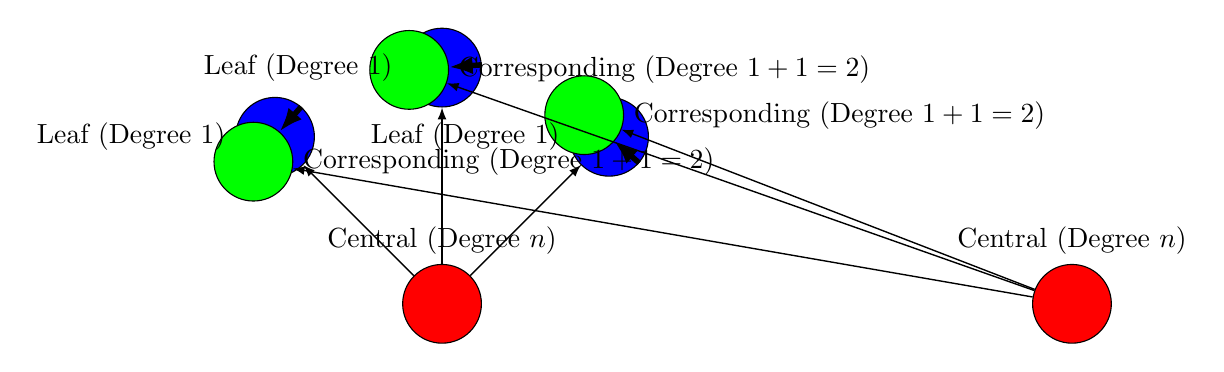
\begin{tikzpicture}[
    vertex/.style={circle, draw, minimum size=1cm, inner sep=0pt},
    central/.style={vertex, fill=red},
    leaf/.style={vertex, fill=blue},
    corresponding/.style={vertex, fill=green},
    double line/.style={black, line width=2pt, -{Latex[length=3mm]}},
    single line/.style={black, line width=0.5pt, -{Latex[length=1.5mm]}}
]
    % First star graph (S_{1,n})
    \node[central] (c1) at (0, 0) {};
    \foreach \i in {1,2,3} {
        \node[leaf] (l1\i) at (45*\i:3cm) {};
        \draw[single line] (c1) -- (l1\i);
    }
    
    % Second star graph (S_{1,n})
    \node[central] (c2) at (8, 0) {};
    \foreach \i in {1,2,3} {
        \node[corresponding] (l2\i) at (8 + 45*\i:3cm) {};
        \draw[single line] (c2) -- (l2\i);
    }
    
    % Double edges between corresponding vertices
    \foreach \i in {1,2,3} {
        \draw[double line] (l1\i) -- (l2\i);
    }
    
    % Labels for vertices (optional)
    \node[above] at (c1.north) {Central (Degree $n$)};
    \node[above] at (c2.north) {Central (Degree $n$)};
    \foreach \i in {1,2,3} {
        \node[left] at (l1\i.west) {Leaf (Degree $1$)};
        \node[right] at (l2\i.east) {Corresponding (Degree $1+1=2$)};
    }
\end{tikzpicture}
\end{document}